\documentclass[a4paper]{article}
\usepackage[utf8]{inputenc}
\usepackage[colorlinks,allcolors=blue]{hyperref}
\usepackage{graphicx}


\title{AI articles on Medium}
\author{paddy10tellys }
\date{October 2019}

\begin{document}

\maketitle

\section{Setting it all up}

I plan to write articles about AI on \href{https://medium.com/}{medium.com} using \hyperlink{https://www.python.org/}{Python3}, \hyperlink{https://www.anaconda.com/}{Anaconda},   \href{https://www.latex-project.org/}{LaTeX}, \href{https://overleaf.com}{overleaf}, \hyperlink{https://colab.research.google.com/notebooks/welcome.ipynb}{colab}, \hyperlink{https://jupyter.org/}{jupyter}, \hyperlink{https://github.com/}{github}, \hyperlink{https://gist.github.com/}{github gists} and other industry-standard tools. This will involve getting down and dirty with calculus, linear algebra and differential equations in mathematical Python. Since GitHub supports rendering of LaTeX equations in jupyter notebooks, all I need to do is write the math in overleaf, transfer it into a colab notebook and then upload it as a gist. Then I can embed it into a medium article. This is a very steep learning curve. If I conquer it then I will be an AI ninja!

\section{LaTeX}

When the \LaTeX\ interpreter processes an input file, it expects it to follow a certain \href{https://en.wikibooks.org/wiki/LaTeX/Document_Structure}{document structure.} Leading backslashes indicate typesetting commands and the curly braces are arguments.

\noindent
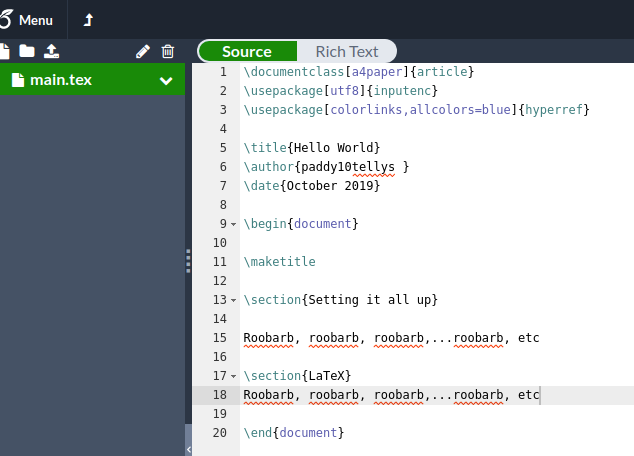
\includegraphics[width=\linewidth]{4.png}


The \textbf{\emph{preamble}} is all of the commands between the the command specifying the document class and the command that specifies where the document begins. Line 1 specifies the the document to be an A4 sized article. Line 2 gives it the means to handle unicode (non ASCII) characters. Line 3 provides the means to format \href{https://en.wikibooks.org/wiki/LaTeX/Hyperlinks}{hyperlinks} by loading the hyperref package \verb+\usepackage{hyperref}+ using the \verb+\usepackage+ command. 

The \verb+href+ command expects a url and text inside separate curly braces. I trawled stackoverflow  \href{https://stackoverflow.com/questions/30421368/latex-how-to-quote-command}{for this post} on, "how to quote a command in LaTeX" to discover that quoting a command requires using the \verb+\verb+ command followed by the actual command between containing delimiters, (usually + or |). All of that just for this one simple paragraph! 

It should be obvious by now that this article is aimed at beginners, is written by a beginner, is learning by doing and is an exploratory ride through the reflective learning cycle. Well, my take on it anyway, naive as it is... I'm doing this alone. The world wide web will have to be my teacher, my audience and hopefully lead to connections with other active learners.

\section{Workflow}
A cyclical sequence of activities: describing, feeling, evaluating, analysing, concluding and action planning.... mainly.

Starting up overleaf opens the projects page. Projects are one of three options positioned on the right end of the menu bar located at the top of the page. The other two being Help and Account. Thankfully, I can sync overleaf to github by going to Account/Account Settings/Github integration even though I'm using a free personal account. Cool!

\noindent
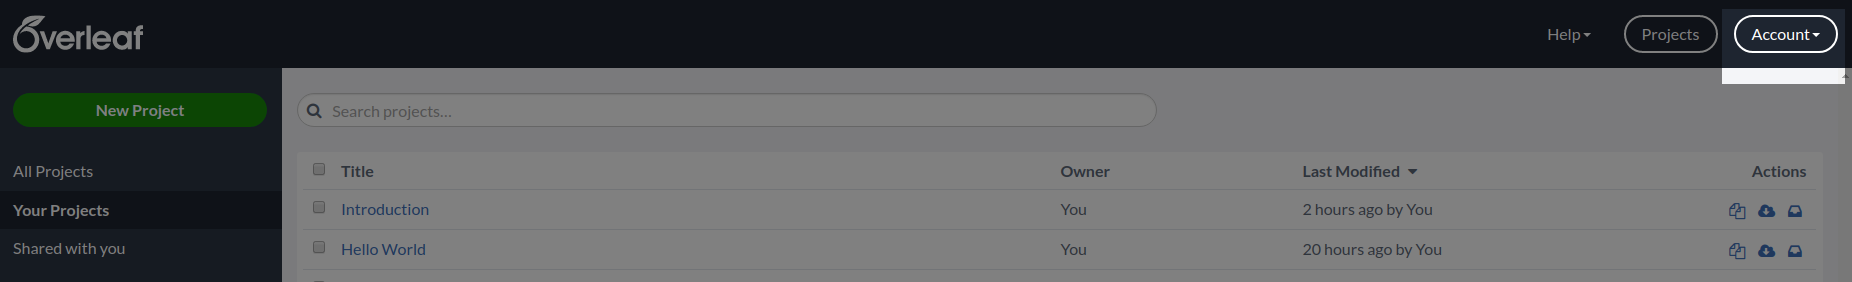
\includegraphics[width=\linewidth]{overleafmenubar.png}



%$ \int_a^b f(x) = F(b) - F(a) $
\end{document}
